\documentclass[11pt]{article}
\usepackage[margin=0.85in]{geometry}
\usepackage{amsmath,amssymb}
\usepackage{graphicx}
\usepackage{booktabs}
\usepackage{array}
\usepackage{xcolor}
\usepackage{titlesec}
\usepackage{enumitem}
\usepackage[hidelinks]{hyperref}
\definecolor{good}{RGB}{20,120,60}
\definecolor{bad}{RGB}{180,40,40}
\definecolor{hdr}{RGB}{25,25,25}
\titlespacing*{\section}{0pt}{1.4ex}{0.6ex}
\titleformat{\section}{\large\bfseries\color{hdr}}{}{0pt}{}
\setlength{\parindent}{0pt}\setlength{\parskip}{0.7ex}
\newcommand{\g}[1]{\textcolor{good}{\textbf{#1}}}
\newcommand{\rd}[1]{\textcolor{bad}{#1}}
\newcommand{\dft}{{\small(Default)}}
\newcommand{\oth}{{\small(others)}}
\newcommand{\ours}{{\small(ours)}}
\pagestyle{empty}

\begin{document}

\begin{center}
{\LARGE\bfseries Progress report --- Value Learning}
\end{center}
\vspace{0.6em}

A model-based agent plans by \emph{imagining} the future: it rolls a learned world-model forward over many
candidate action sequences and keeps the one whose imagined endpoint $\hat z_{t+H}$ --- a vector, the
model's compressed ``state,'' or \emph{latent} --- is \textbf{closest} to the goal $z_g$. Everything hinges
on what ``closest'' means: the \textbf{plan score} we assign to each candidate's imagined endpoint
$(\hat z_{t+H},\,z_g)$.

\begin{center}
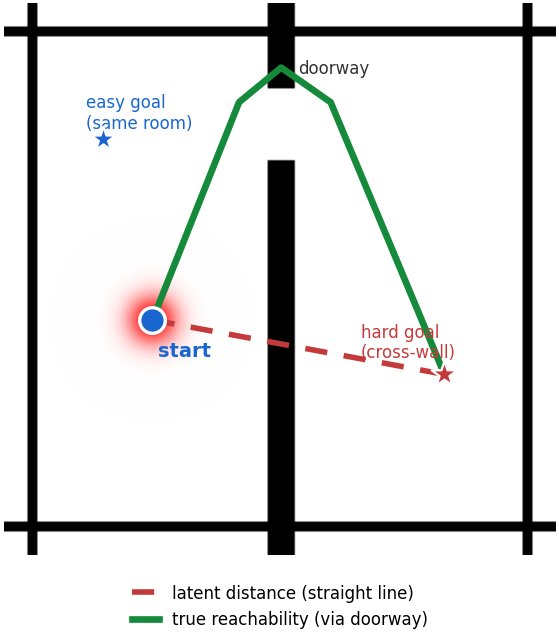
\includegraphics[width=0.42\textwidth]{tworoom_fig.png}
\\[0.2em]
\begin{minipage}{0.86\textwidth}
{\small\textbf{The benchmark, \textsf{TwoRoom}:} two rooms joined by one doorway. \emph{Easy} goals sit in the
same room; \emph{hard} goals are across the wall. The \textcolor{bad}{straight latent distance} points
through the wall, while \textcolor{good}{true reachability} must detour through the doorway.}
\end{minipage}
\end{center}

\section{The default plan score --- and why it is wrong}
Today's latent world-model planners --- \textsf{LeWM}, \textsf{DINO-WM}, \textsf{PLDM} --- all score
closeness with the \emph{latent distance} $\lVert \hat z_{t+H}-z_g\rVert^2$ (plain Euclidean distance in
latent space). \textbf{The catch: this distance is never trained to represent actual distance.} It simply
falls out of a model trained to \emph{predict frames}, so nothing forces it to track \emph{how far to walk}.
A goal on the far side of a wall looks ``near'' in latent space yet is many steps away --- the straight line
cuts through the wall (above), so the planner steers into it. We test four plan scores on this benchmark, on
easy and hard goals, giving every one the \emph{same} planning budget; we report the \% of 100 goals reached.

\section{The four plan scores we compare}
\begin{itemize}[leftmargin=1.4em,itemsep=0.7ex,topsep=0.4ex]
\item \textbf{Latent distance \dft} $=\lVert \hat z-z_g\rVert$ --- the current standard. Free, no training;
completely blind to obstacles.
\item \textbf{Regression --- ``TRM'' \oth} --- the prior published metric: a network trained (supervised) to
predict the step-gap between two states drawn from logged trajectories. Better than raw distance, but it only
knows the paths the data \emph{happened} to take --- if they wandered, it learns inflated distances, and it
cannot infer a shortcut it never saw.
\item \textbf{TD value \ours\ --- \emph{value learning}.} Instead of copying observed gaps, learn a
goal-conditioned \emph{value} $d(z,z_g)\!\approx\!$ steps-to-go with a Bellman / temporal-difference update,
$d(z,g)\leftarrow 1+\min_{z'} d(z',g)$. The $\min$/bootstrap \textbf{stitches} short transitions
into the globally \emph{shortest} path, so even from non-optimal data it recovers true reachability and finds
the route through the doorway. (Our one-line fix lives here: the bootstrap must be \emph{optimistic} --- take
the shortest stitched path, not the average.)
\item \textbf{Online TD \ours\ --- \emph{self-practice}.} Let the planner act with the current value $d$,
collect those rollouts, and keep training $d$ on them --- so the score becomes accurate exactly on the states
the planner actually visits (which a fixed log under-covers).
\end{itemize}

\section{Results: \% of goals reached}
\begin{center}
\renewcommand{\arraystretch}{1.4}
\setlength{\tabcolsep}{5pt}
\begin{tabular}{ll cccc}
\toprule
 & & \textbf{Latent dist.} & \textbf{TRM} & \textbf{TD value} & \textbf{Online TD} \\
\textbf{World model} & \textbf{Goals} & \dft & \oth & \ours & \ours \\
\midrule
\textsf{DINO-WM} & easy & 71 & 58 & \g{95} & 95 \\
\textsf{DINO-WM} & \textbf{hard} & \rd{34} & 29 & 83 & \g{93} \\
\addlinespace[3pt]
\textsf{LeWM}    & easy & 78 & 62 & \g{92} & 90 \\
\textsf{LeWM}    & \textbf{hard} & \rd{16} & 29 & 64 & \g{68} \\
\bottomrule
\end{tabular}
\end{center}
{\small \emph{Green} $=$ best plan score in that row;\; \textcolor{bad}{red} $=$ the default score collapsing
on hard goals.\; A perfect-knowledge planner scores $\approx$100\%.}

\section{What it means}
\begin{itemize}[leftmargin=1.4em,itemsep=0.8ex,topsep=0.4ex]
\item \textbf{On hard goals the default score all but fails} (\rd{16--34\%}), and the prior metric (TRM)
barely helps (29\%, even trailing the default on \textsf{DINO}) --- copying observed gaps isn't the same as
finding shortest paths.
\item \textbf{Value learning (TD) is the jump} (hard: $16\!\to\!64$, $34\!\to\!83$). And the
\emph{optimistic-target fix} alone roughly doubled hard-goal success ($52\!\to\!64$, $65\!\to\!83$) --- a
one-line change to the training objective.
\item \textbf{Self-practice adds the last mile} (\textsf{DINO} $83\!\to\!\g{93}$, \textsf{LeWM}
$64\!\to\!\g{68}$) --- and it is the practice \emph{data}, not extra compute: training the offline value
$2\times$ longer instead over-fits and gets \emph{worse} ($83\!\to\!73$, $64\!\to\!60$).
\end{itemize}

\vspace{1.4em}
{\footnotesize\color{gray}
\textbf{Details.} Hard / easy $=$ the n100 goal set at geodesic $90$--$180$ / $20$--$70$\,px (50 cross-wall
$+$ 50 same-room). Matched budget $=$ CEM $30\times5\approx150$ candidate evaluations. TD value $=$ offline
goal-conditioned temporal-difference on a quasimetric head; the ``optimistic'' setting is the TD
\emph{expectile} ($\tau\!<\!0.5$, biased toward the shortest path). Self-practice $=$ the same value
continued online on planner-collected rollouts; the gain was verified against a matched-compute control.}

\end{document}
